\chapter{非正交的Wannier插值方法}

Wannier函数包含了一个能带的所有信息。不仅如此,由于Wannier函数非常局域,它们可以仅仅用倒空间的很少的一部分$\bk$点构造出来\cite{souza_maximally-localized_2001,marzari_maximally_1997}。在得到Wannier函数之后,任意$\bk$点的本征布洛赫波函数都可以通过一个简单的傅里叶变换求得,这个过程叫做Wannier插值\cite{marzari_maximally_2012}。Wannier插值抓住了布洛赫电子的本质,是一个计算各种物理可观测量的高效的方法。之前的研究将Wannier插值应用在了反常霍尔电导\cite{wang_textitab_2006},介电常数\cite{yates_spectral_2007},轨道磁矩\cite{lopez_wannier-based_2012}以及包括位移电流\cite{wang_first-principles_2017,ibanez-azpiroz_ab_2018}和倍频效应\cite{wang_first-principles_2017}的二阶光学效应中。


目前的构造Wannier函数的流行算法是最大局域化Wannier函数算法,这个算法将能带混合在一起,通过调整混合的方式将Wannier函数的展宽尽量减小\cite{marzari_maximally_2012}。这个方法非常普适,经常被作为各种第一性原理计算软件包的后处理工具\cite{mostofi_updated_2014},并且处理方法和第一性原理软件的实现方式几乎无关。但是,由于最大局域化Wannier函数算法本质上是最优化算法,为了避免局域最小,初始的猜测Wannier函数以及很多其他参数都需要小心的测试。这个过程不可避免的需要人的参与,因此在高通量计算中不太适用。而且,在优化Wannier函数的过程中对称性一般会被破坏,这些对称性在材料性质,比如非线性光学效应和拓扑性质中,往往起着重要的作用。一个解决这些问题的方案是采用基于实空间局域基组的密度泛函计算方法,很多的第一性原理计算软件包已经采用了这样的计算方法。但是,一个非常重要的事实是绝大部分采用实空间局域基组的第一性原理计算软件包都用的是非正交的局域基组。这个做法主要有两个原因:(一)非正交局域基组一般而言没有长尾效应,能够做得更加局域。(二)构造大量的非正交局域基组更加容易。目前的Wannier插值方法都是假设Wannier函数是正交的,因此不能够直接用于非正交局域基组。因此,将Wannier插值方法推广到非正交局域基组就显得非常必要。

本章我们将发展一个基于非正交局域基组的广义的Wannier插值方法。这个方法可以计算能带能量和相应布洛赫波函数的任意阶导数。因此,这个方法适合用来计算多种线性和非线性响应函数。我们以WS$_2$的介电常数和位移电导为例,作为这个方法可以计算线性和非线性响应的例子。我们得到的结果和之前的工作是完全一致的。最后,我们讨论了这个方法的性能和对称性相关的性质。

\section{计算方法}\label{sec:method}

贝里联络\cite{berry_quantal_1984} $\boldsymbol{\berry}_{nm}(\boldsymbol{k})=i\langle u_{n\boldsymbol{k}}|\nabla_{\boldsymbol{k}}u_{m\boldsymbol{k}}\rangle$及其导数$\nabla_{\boldsymbol{k}}\boldsymbol{\berry}$是计算响应函数的核心。但是,由于矩阵对角化会引入随机相位,直接的有限差分方式并不适用。Wannier插值方案通过选择一个确定的相位规范来解决这个问题。这里,我们将这个方案推广到非正交局域基组。

我们用 $|\boldsymbol{R}n\rangle$来标记局域轨道,这里$n$是元胞内的轨道的标记,$\boldsymbol{R}$是元胞的标记。 $n$取值从$1$到$N$, 这里$N$是一个元胞内的轨道数目。这些轨道的布洛赫求和就构成了哈密顿量在一个$\bk$点的一组完备基,
\[
|\psi_{n\boldsymbol{k}}^{(\text{W})}\rangle\equiv\sum_{\boldsymbol{R}}e^{i\boldsymbol{k}\cdot\boldsymbol{R}}|\boldsymbol{R}n\rangle
\]
布洛赫波的周期性部分是 
\[
|u_{n\boldsymbol{k}}^{(\text{W})}\rangle\equiv e^{-i\boldsymbol{k}\cdot\hat{\boldsymbol{r}}}|\psi_{n\boldsymbol{k}}^{(\text{W})}\rangle=\sum_{\boldsymbol{R}}e^{i\boldsymbol{k}\cdot(\boldsymbol{R}-\hat{\boldsymbol{r}})}|\boldsymbol{R}n\rangle.
\]
在这组基下,哈密顿量的表示矩阵元是
\begin{align}
\begin{split}
H_{nm}(\boldsymbol{k}) & \equiv\langle\psi_{n\boldsymbol{k}}^{(\text{W})}|\hat{H}|\psi_{m\boldsymbol{k}}^{(\text{W})}\rangle\\
& =\sum_{\boldsymbol{R}}e^{i\boldsymbol{k}\cdot\boldsymbol{R}}\langle\boldsymbol{0}n|\hat{H}|\boldsymbol{R}m\rangle,
\end{split}
\end{align}
和普通的Wannier插值方法不一样的是,$|\psi_{n\boldsymbol{k}}^{(\text{W})}\rangle$一般而言既不相互正交,也没有归一化。因此,需要一个交叠矩阵来描述这个行为,
\begin{align}
\begin{split}
S_{nm}(\boldsymbol{k}) & \equiv\langle\psi_{n\boldsymbol{k}}^{(\text{W})}|\psi_{m\boldsymbol{k}}^{(\text{W})}\rangle\\
& =\sum_{\boldsymbol{R}}e^{i\boldsymbol{k}\cdot\boldsymbol{R}}\langle\boldsymbol{0}n|\boldsymbol{R}m\rangle.\label{S}
\end{split}
\end{align}
哈密顿量$\hat{H}$的本征态是$|\psi_{n\boldsymbol{k}}^{(\text{W})}\rangle$的线性叠加,
\begin{align}
|\psi_{n\boldsymbol{k}}\rangle & =\sum_{m}V_{mn}(\boldsymbol{k})|\psi_{m\boldsymbol{k}}^{(\text{W})}\rangle,\\
\hat{H}|\psi_{n\boldsymbol{k}}\rangle & =E_{n\boldsymbol{k}}|\psi_{n\boldsymbol{k}}\rangle,
\end{align}
这里$V$和$E$可以通过计算一个广义的本征值问题来求得,
\begin{equation}
H(\boldsymbol{k})v_{n\boldsymbol{k}}=E_{l\boldsymbol{k}}S(\boldsymbol{k})v_{n\boldsymbol{k}}.\label{eq:gep}
\end{equation}
上式仅仅是薛定谔方程在非正交基$|\psi_{n\boldsymbol{k}}^{(\text{W})}\rangle$下的表示。 $v_{n\boldsymbol{k}}$ 是一个列向量,有$N$个线性独立的解,这些解构成了$V$的列。值得注意的是$V$不是一个幺正矩阵。我们假设非正交局域基是线性无关的,那么$S$既是正定的,也是厄米的。这样的广义本征值问题的行为很好,并且本征矢可以按下面的式子归一。
\begin{equation}
v_{n}^{\dagger}Sv_{m}=\delta_{nm}.\label{eq:norm}
\end{equation}

贝里联络可以用$V$表示出来,
\begin{equation}
\berry^{\alpha}=iV^{\dagger}S\partial_{\alpha}V+V{}^{\dagger}\berry^{\alpha(\text{W})}V,\label{eq:A}
\end{equation}
这里
\begin{align}
\begin{split}
\berry_{nm}^{\alpha(\text{W})} & \equiv i\langle u_{n\boldsymbol{k}}^{(\text{W})}|\partial_{\alpha}u_{m\boldsymbol{k}}^{(\text{W})}\rangle\\
& =\sum_{\boldsymbol{R}}e^{i\boldsymbol{k}\cdot\boldsymbol{R}}(\langle\boldsymbol{0}n|\hat{r}^{\alpha}|\boldsymbol{R}m\rangle-R^{\alpha}\langle\boldsymbol{0}n|\boldsymbol{R}m\rangle)
\end{split}
\end{align}
$\hat{r}$ 是位置算符,$\partial_{\alpha}\equiv\partial_{k^{\alpha}}$,$\alpha$是笛卡尔指标。对非正交局域基,位置算符可以写为
\begin{align}
\begin{split}
\langle\boldsymbol{0}m|\hat{r}^{\alpha}|\bar{\boldsymbol{R}}n\rangle & =(\langle\bar{\boldsymbol{R}}n|\hat{r}^{\alpha}|\boldsymbol{0}m\rangle)^{*}\\
& =(\langle\boldsymbol{0}n|\hat{r}^{\alpha}|\boldsymbol{R}m\rangle)^{*}-R^{\alpha}\langle\boldsymbol{0}m|\bar{\boldsymbol{R}}n\rangle,
\end{split}
\end{align}
这里$\bar{\boldsymbol{R}}=-\boldsymbol{R}$。
与此相反的是,在基于最大局域化Wannier函数的Wannier插值方法中,$\langle\boldsymbol{0}m|\hat{r}^{\alpha}|\boldsymbol{R}n\rangle$ (在固定 $\boldsymbol{R}$的情况)下是一个厄米矩阵。 

但是,计算$V^{\dagger}S\partial_{\alpha}V$仍然会遇到随机相位的问题,因为$V$仍然是对角化得到的。幸运的是,由于$\langle\boldsymbol{0}n|\hat{H}|\boldsymbol{R}m\rangle$,
$\langle\boldsymbol{0}n|\boldsymbol{R}m\rangle$和$\langle\boldsymbol{0}n|\hat{r}^{\alpha}|\boldsymbol{R}m\rangle$这三个矩阵可以从第一性原理求得,$H$, $S$ 和 $\berry^{(\text{W})}$的任意阶导数都可以得到。这样,计算 $V^{\dagger}S\partial_{\alpha}V$ \cite{van2007computation}便成为了可能。这里,我们在$\Gamma$点 ($\boldsymbol{k}=\boldsymbol{0}$)计算
$V^{\dagger}S\partial_{\alpha}V$作为一个例子。对式\ref{eq:gep}两边微分,可以得到
\begin{align}
\begin{split}
(\partial_\alpha H)v_n+H\partial_\alpha v_n = & (\partial_\alpha E_n)Sv_n+\\
& E_n(\partial_\alpha S)v_n+E_n S(\partial_\alpha v_n).\label{eq:dgep}
\end{split}
\end{align}
将式\ref{eq:dgep}左乘$v_{n}^{\dagger}$,可以得到
\[
\partial_\alpha E_{n}=v_{n}^{\dagger}(\partial_\alpha H) v_{n}-E_{n}v_{n}^{\dagger}(\partial_\alpha S)v_{n}.
\]
将式(\ref{eq:dgep})左乘$v_{m}^{\dagger}$ ($m\ne n$),可以得到
\[
v_{m}^{\dagger}S\partial_\alpha v_{n}=\frac{v_{m}^{\dagger}(\partial_\alpha H)v_{n}-E_{n}v_{m}^{\dagger}(\partial_\alpha S)v_{n}}{E_n-E_m}.
\]
但是,由于$v_{n}$存在着本征的相位不确定性,我们需要引入一个相位规范来得到$v_{n}^{\dagger}S \partial_\alpha v_{n}$,
\begin{equation}
v_{n\boldsymbol{0}}^{\dagger}S(\boldsymbol{0})v_{n\boldsymbol{k}}\in\mathbb{R}。\label{eq:phase}
\end{equation}
由于$v_{n\boldsymbol{0}}^{\dagger}S(\boldsymbol{0})v_{n\boldsymbol{0}}=1\in\mathbb{R}$,这个规范在$\Gamma$点是平滑的。将式\ref{eq:norm}和式\ref{eq:phase}都微分,可以得到
\[
v_{n}^{\dagger}S\partial_\alpha v_n=-\frac{1}{2}v_{n}^{\dagger}(\partial_\alpha S)v_n.
\]
在上面的推导中,我们假设了$n$不是简并的。原则上简并的能级也可以处理\cite{andrew1998computation},但是这个在我们当前的计算中并不重要。

现在我们已经可以计算线性响应了。但是,如果要计算非线性响应,我们还需要求得$\nabla_{\boldsymbol{k}}\boldsymbol{\berry}$。 对式Eq. (\ref{eq:A})进一步求导,我们得到
\begin{equation}
\begin{split}
\partial_{\beta}\berry^{\alpha}  = &i(\partial_{\beta}V^{\dagger})S(\partial_{\alpha}V)+iV^{\dagger}(\partial_{\beta}S)(\partial_{\alpha}V)\\
&+iV^{\dagger}S\partial_{\beta}\partial_{\alpha}V+(\partial_{\beta})V^{\dagger}\berry^{\alpha(\text{W})}V\\
&+V^{\dagger}(\partial_{\beta}\berry^{\alpha(\text{W})})V+V^{\dagger}\berry^{\alpha(\text{W})}(\partial_{\beta}V).
\end{split}
\end{equation}
如果是正交的Wannier函数\cite{wang_first-principles_2017},我们只需要在上式中将$S$设为$I$。 $V^{\dagger}S\partial_{\beta}\partial_{\alpha}V$的计算和$V^{\dagger}S\partial_{\alpha}V$的计算遵循相似的逻辑。但是不难想象,最后的表达式应该非常复杂。因此,我们在\app{app:degep}中介绍一种递归的计算方法,这个方法可以得到$v_n$和$E_{n}$的任意阶导数。


另外一个计算贝里相位的办法是对\ref{eq:gep}采用 $S^{-1/2}$进行正交化,然后采用传统的Wannier插值方法进行计算。但是由于Wannier插值需要正交化过的哈密顿量的任意阶导数,这个方法需要求得对$S^{-1/2}$的任意阶导数。这个方法将在\s{sec:orthogonalization}里面阐释。

既然我们已经得到了线性和非线性响应函数的所需要矩阵元,我们下面对单层WS$_2$的介电常数和位移电导进行计算,并且和之前的工作进行对比。

\section{单层WS$_2$的位移电流}

\begin{figure}
    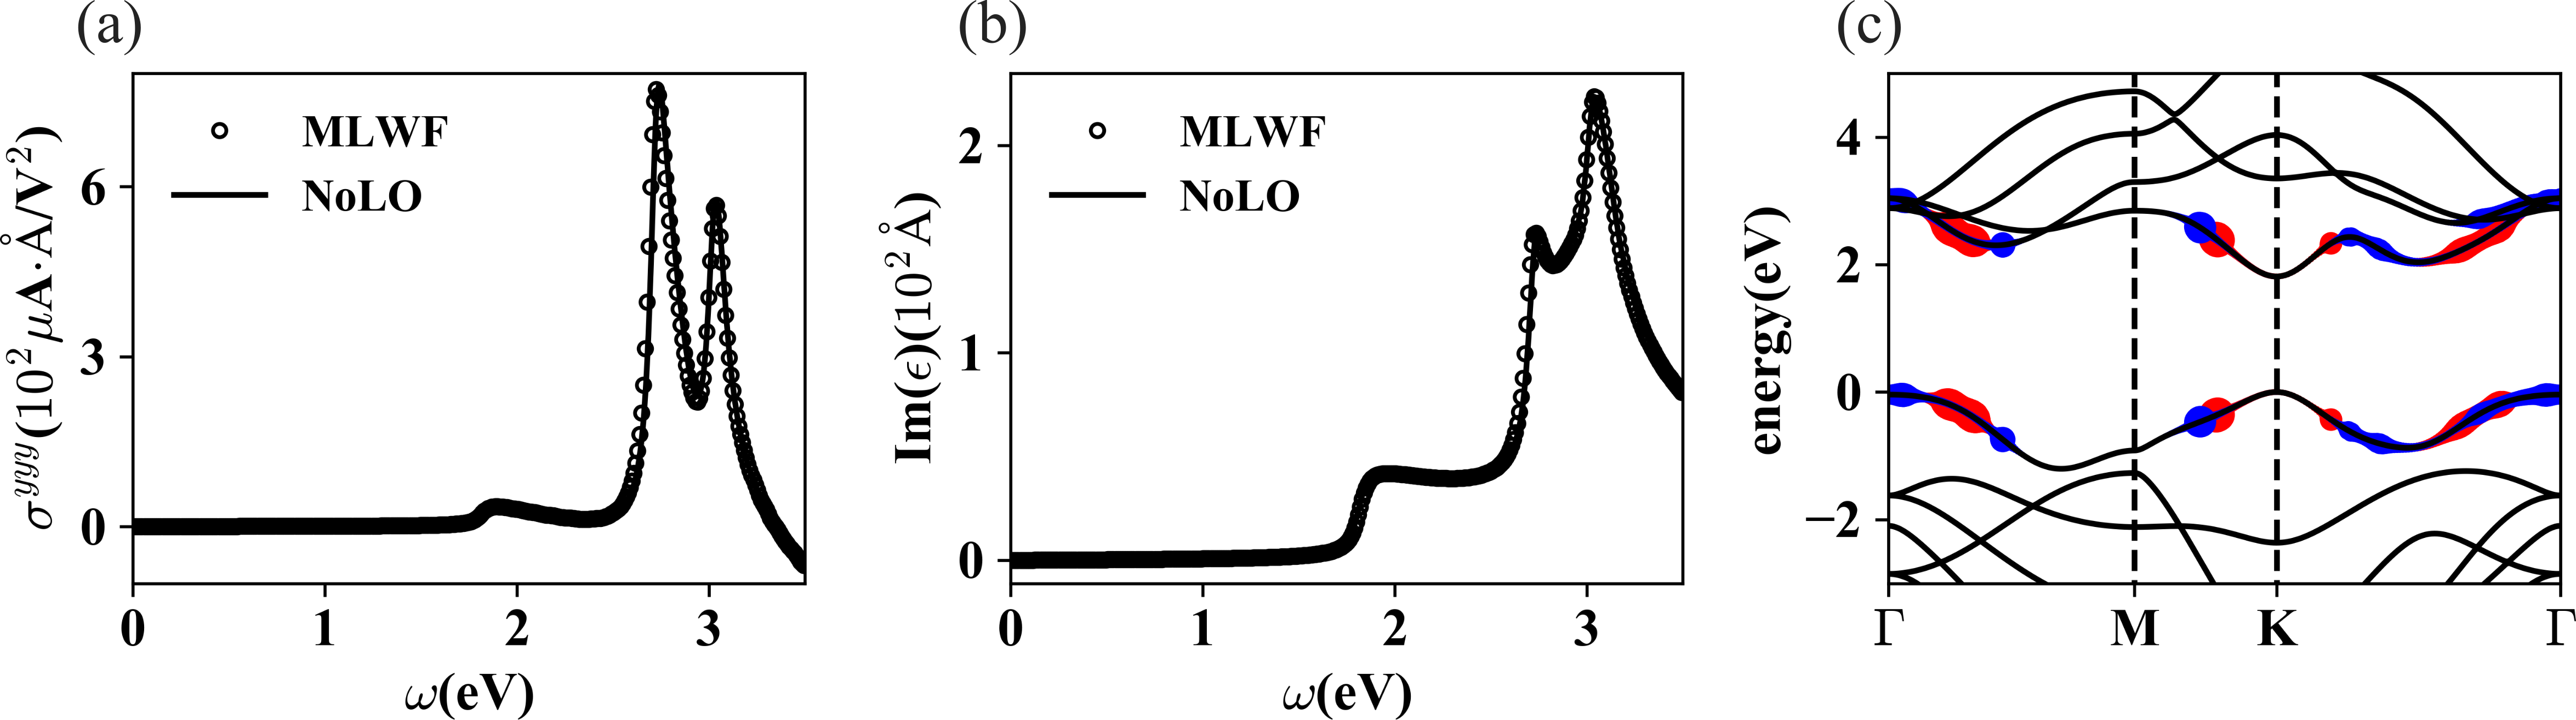
\includegraphics[width=1.0\textwidth]{WS2.png}
    \centering
    \caption{单层WS$_2$的位移电导。(a)基于最大局域化Wannier函数和非正交局域轨道的Wannier插值方法计算的位移电流。(b)基于最大局域化Wannier函数和非正交局域轨道的Wannier插值方法计算的介电常数的虚部。第一个峰和第二个峰的贡献画在了能带图(c)中。第一个峰是红色的点,第二个峰是蓝色的点,点的大小对应贡献的大小。\label{fig:WS2}}
\end{figure}

\subsection{计算方法}

由于单层 WS$_2$的点群是$D_{6h}$,位移电导只有一个独立的,不为零的分量 $\sigma^{yyy}$\cite{bilbao,wang_first-principles_2017}。根据文献\onlinecite{wang_first-principles_2017}的惯例,我们采用二维电流密度的定义。我们的第一性原理计算采用了一个全电子的软件包\textsc{fhi-aims}。电子的交换关联作用采用了PBE泛函\cite{perdew_generalized_1996}来处理。我们采用一个层状模型来模拟单层WS$_2$,其中真空层的厚度超过了15\AA。在自洽计算中,我们采用了$12\times12\times1$的$\bk$点来进行布里渊区的积分。但是在计算位移电流的时候,我们采用了密得多的$400\times400\times1$的$\bk$点进行数值积分。在\textsc{fhi-aims}数值积分中,我们采用了“tight”的数值设定,这个设定足以保证原子轨道基矢能够充分地展开Kohn-Sham波函数,并且实空间积分的格点也能够收敛\cite{blum_ab_2009}。我们没有引入自旋轨道耦合。在计算中,我们采用了$\delta$函数的近似
\[
\delta(x)=\lim_{\epsilon\to0}\frac{1}{\pi}\frac{\epsilon}{\epsilon^2+x^2},
\]
这里展宽因子$\epsilon$取为$0.04$eV.


\subsection{结果}

\fig{fig:WS2}里展示了单层WS$_2$的位移电导。这个结果和之前工作\onlinecite{wang_first-principles_2017}中基于最大局域化Wannier函数的Wannier插值结果在相同参数情况下进行了对比。我们可以看到,尽管我们采用了不同的软件包,不同的DFT实现方式,两种方式计算得到的位移电导的曲线几乎完全重合。除此之外,我们还采用基于最大局域化Wannier函数和基于非正交局域函数的Wannier插值方法计算了光学吸收,也就是介电函数的虚部,这个结果展示在\fig{fig:WS2}中。介电函数和位移电导的曲线都有两个峰,一个峰在2.75eV,另外一个峰在3.05eV。尽管介电函数在3.05eV处的峰高于2.75eV处的峰,位移电导的特征却正好相反。这个差别应该是由位移矢量的不同导致的。在\fig{fig:WS2}中,我们将这两个峰的贡献分解在了能带上,红色和蓝色的点的大小体现了这个点对2.75eV和3.05eV处的峰的贡献大小。我们从图中可以看出这两个峰都是由最高的价带和最低的四条导带在$\Gamma$和$K$点附近贡献的。


\subsection{关于方法的讨论}

我们已经知道,最大局域化Wannier函数在构造过程中一般会轻微破坏对称性,这一点体现在本应简并的能带在Wannier插值的时候出现一个很小的带隙。在位移电导上,这个特征体现在即使Wannier函数构造的时候收敛良好,被对称性禁戒的分量计算的时候也会得到不为零的值。但是,由于仅仅不可约布里渊区中的点才会被积分,基于非正交局域函数的第一性原理软件不会出现这样的问题。我们在\fig{fig:performance}中展示了用最大局域化Wannier函数和非正交局域基组计算的单层WS$_2$的$\sigma^{xxx}$分量,这个分量是被对称性禁戒的。我们可以看到基于最大局域化Wannier函数的方法有一个1$\mu$A$\cdot$\AA/V$^2$左右的值,而基于非正交局域基组的Wannier插值则基本为零(不大于)$10^{-4}\mu$A$\cdot$\AA/V$^2$。从这个角度看,基于非正交局域基组的Wannier插值能够很好的保持对称性。

第一性原理计算,尤其是全电子的第一性原理计算,一般需要采用大量的轨道来展开希尔伯特空间,与此相反,最大局域化Wannier函数则仅仅需要在费米面附近构造,因此,计算中我们非正交局域基组的数量往往远超Wannier函数的数目。从这个角度来讲,本章提出的方法计算量更加大一些。在这样的情况下,我们测试了计算时间和非正交局域基组数量的关系。我们发现,计算时间基本上和非正交局域基组的数目的关系是$\text{O}(N^2)$,这里$N$是非正交局域基组的数目(见\fig{fig:performance})。这一点是比较奇怪的,因为对角化的计算复杂度往往是$\text{O}(N^3)$。进一步的分析表明,绝大部分计算计算时间用在了变换,也就是计算$H$, $S$, $A^{(\text{W})}$及其导数上。因此,对于正常大小的体系,我们可以简单的认为计算复杂度就是$\text{O}(N^2)$。

\begin{figure}
    \includegraphics[width=0.9\textwidth]{performance.png}
    \centering
    \caption{(a)单层WS$_2$对称性禁戒的位移电流分量的计算。(b)计算时长和轨道数目($N$)的关系。黑色的点是实际的数据,线是拟合的结果,线的斜率基本是2。\label{fig:performance}}
\end{figure}

\section{正交化方案}\label{sec:orthogonalization}

尽管$|\psi^{(\text{W})}_{n\boldsymbol{k}}\rangle$不是正交的,我们可以利用正交化得到一组正交的基:
\begin{equation}
|\psi^{(\text{O})}_{n\boldsymbol{k}}\rangle=
\sum_m |\psi^{(\text{W})}_{m\boldsymbol{k}}\rangle S^{-1/2}_{mn}(\boldsymbol{k}).
\end{equation}
在这组正交基下,哈密顿量$H^{(\text{O})}(\boldsymbol{k})$和$H^{(\text{W})}(\boldsymbol{k})$的关系是
\begin{equation}
H^{(\text{O})}(\boldsymbol{k})=S^{1/2}(\boldsymbol{k})H^{(\text{W})}(\boldsymbol{k})S^{-1/2}(\boldsymbol{k}).\label{HO-HW}
\end{equation}
由于$S(\boldsymbol{k})$是正定的,因此$S(\boldsymbol{k})$的开根号是有着良好定义的。通过以上的变换,基于最大局域化Wannier函数的方法就可以直接用在非正交局域基组上。

但是,在基于最大局域化Wannier函数的Wannier插值中,哈密顿量$H^{(\text{O})}(\boldsymbol{k})$对$\bk$的任意阶导数是一个非常重要的组成部分。从式\ref{HO-HW}中,我们可以看出这个问题简化为求解$S^{-1/2}(\boldsymbol{k})$对$\bk$的任意阶导数。这个导数可以如下求得。通过两边求导$S^{-1/2}S^{-1/2}=S^{-1}$,我们得到
\begin{equation}
(\partial_{\alpha}S^{-1/2})S^{-1/2}+S^{-1/2}\partial_{\alpha}S^{-1/2}=\partial_{\alpha}S^{-1}.\label{dS1/2-1}
\end{equation}
其中的$\partial_{\alpha}S^{-1}$可以通过对$SS^{-1}=I$两边求导得到,
\begin{align}
(\partial_{\alpha}S)S^{-1}+S\partial_{\alpha}S^{-1}=0
\end{align}
结果是
\begin{align}
\partial_{\alpha}S^{-1} = -S^{-1}(\partial_{\alpha}S)S^{-1}.
\end{align}

式\ref{dS1/2-1}是一个Sylvester方程\cite{sylvester},在$S$是正定的情况下,这个方程有且仅有一个解。这个解可以用已有的代码得到\cite{laug},它就是所需要求得的$S^{-1/2}(\boldsymbol{k})$的一阶导数。如果我们将$S^{-1/2}S^{-1/2}=S^{-1}$求导到二阶,也可以通过类似的方法求得$S^{-1/2}(\boldsymbol{k})$的二阶导数。不难想象,通过类似的方法,$S^{-1/2}(\boldsymbol{k})$的任意阶导数都可以求得。


这一节所述的正交化的方法的优势是和已有的基于最大局域化Wannier函数的插值方法存在着直接联系。但是,由于这个方法大量的用到了矩阵的求逆,这个方法的计算量略大于\ref{sec:method}的方法,数值稳定性也稍微差一些。


\section{总结}

基于实空间局域基组的第一性原理计算软件有潜力能够实现$\text{O}(N)$的计算量和基组数目的渐进关系。除此之外,这些计算软件中真空层的处理相对简单,不需要增加额外的计算量,在低维材料的计算中用途很大。这里,我们证明了这些软件通过基于非正交局域基组的Wannier插值,可以变得更加强大。

和基于最大局域化Wannier函数的Wannier插值相比,尽管基于非正交基组的Wannier插值的计算量相对较大,但是这个方法可以避免人工干预,可以应用于材料的高通量计算。我们通过计算单层WS$_2$的位移电流,证明了这个方法的正确性和有效性。这个基于非正交局域基的Wannier插值方法非常普适,可以计算各种领域的各种线性和非线性的响应函数\cite{tokura_nonreciprocal_2018},包括反常电导(关于反常电导,可以参见文献\onlinecite{lee_tight-binding_2018}),非线性霍尔效应,轨道磁矩和倍频效应。

